\subsection{Адаптивный геометрический алгоритм}

Прежде всего, следует объяяснить принцип работы геометрического алгоритма.

Геометрический алгоритм опирается на взаимоположение окружностей и их радиусы, и результирующие точки пересечения имеют ключевое значение. На рисунке \ref{fig:scenarios} показаны наиболее часто возникающие сценарии (точки, соответствующие пересечениям окружностей, обозначены как $a, b, c,$ и так далее). 

\begin{figure}
    \centering
    \begin{subfigure}[ht]{0.4\textwidth}
        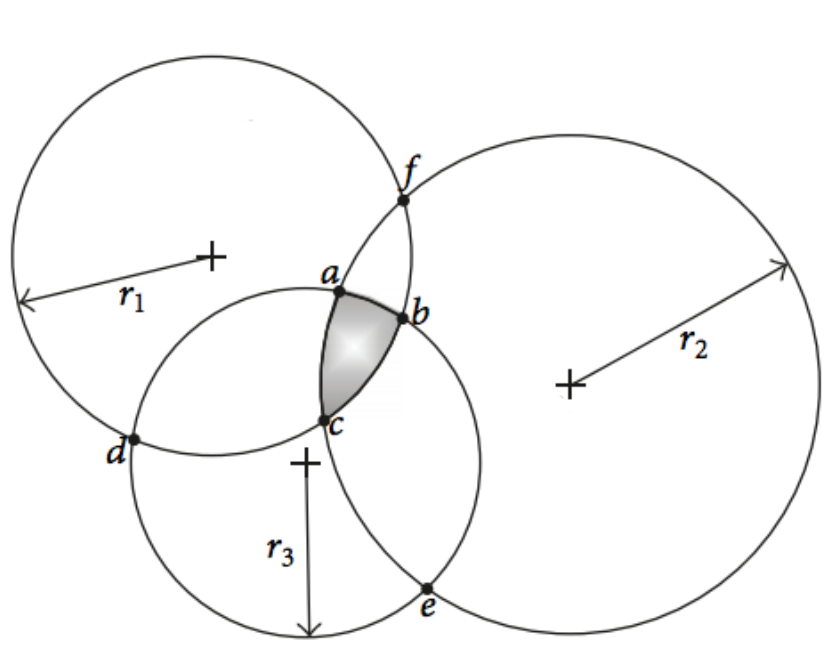
\includegraphics[width=\textwidth]{img/circlesInter}
        \caption{}
        \label{fig:inter}
    \end{subfigure}
    \begin{subfigure}[ht]{0.4\textwidth}
        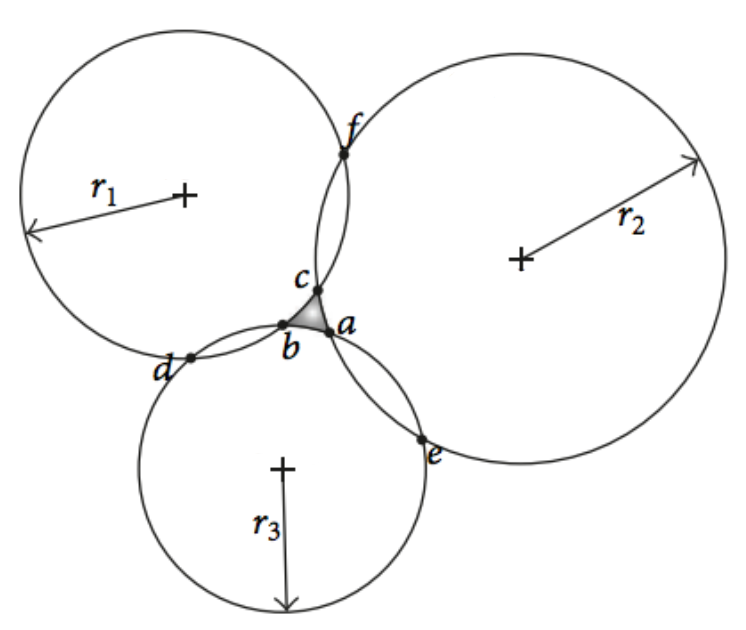
\includegraphics[width=\textwidth]{img/circlesOuter}
        \caption{}
        \label{fig:outer}
    \end{subfigure}
    \caption{Наиболее часто встречающиеся сценарии при работе геометрического алгоритма}
    \label{fig:scenarios}
\end{figure}

В случае, изображенном на рисунке \ref{fig:inter}, нас интересуют только три точки из шести, так как они формируют область, принадлежащую всем трем окружностям.

На рисунке \ref{fig:outer} более сложный сценарий, ведь общей области пересечения всех трех окружностей нет. Следовательно, мы должны воспользоваться другой логикой для нахождения искомой области. Конкретнее, для каждй пары точек, образовавшейся в результате пересечения пары окружностей, нас удовлетворяет та точка, которая находится ближе к третьей окружности (например, из точек $a$ и $e$ будет выбрана $a$, так как она находится ближе к окружности с радиусом $r_1$).

Наконец, искомым положением пользователя является центроид, вычислимый по формуле \ref{for:centroid}.
 
\begin{equation} \label{for:centroid}
    x = \frac{1}{K}\sum^K_{l=1}x_l, \quad y = \frac{1}{K}\sum^K_{l=1}y_l, \quad  l = 1,2,...,K
\end{equation}

$K$ в представленной выше формуле означает количество подходящих точек пересечений. Для случая с тремя окружностями $K=3$.

В работе \cite{brida2013novel} представлена идея \textit{адаптивного геометрического алгоритма}. В сущности, геометрический алгоритм, описанный выше, является частным случаем, а точнее - первой итерацией адаптивного геометрического алгоритма. 

\begin{figure}[ht]
    \centering
    \includegraphics[width=\textwidth]{img/agaDiag}
    \caption{Диаграмма потока данных адаптивного геометрического алгоритма}
    \label{fig:aga}
\end{figure}

Благодаря данной первой итерации получен набор точек пересечения. Суть алгоритма сводится к пропорциональному увеличению или уменьшению всех трех радиусов окружностей так, чтобы общая область пересечений (см. случай на рисунке \ref{fig:inter}) была наименьшей. Конечный этап - нахождение положения пользователя - осуществляется по формуле \ref{for:centroid}. Алгоритм работы проиллюстрирован на рисунке \ref{fig:aga}.

В настоящей работе предложена модификация алгоритма для увеличения скорости его работы. Суть изменения сводится к следующему: для случая, показанного на рисунке \ref{fig:inter}, вместо пропорционального уменьшения радиусов, вычисляются координаты центроида точек пересечения. Для случая, показанного на рисунке \ref{fig:outer}, алгоритм функционирует, как описано выше. 

Полный листинг конечной версии алгоритма представлен в приложении 3.